\documentclass[11pt, xcolor=dvipsnames]{beamer}
\usepackage[latin1]{inputenc}
\usepackage[ngerman]{babel}
\usepackage{amsmath}
\usepackage{lmodern} %f�r mathmode wichtig
\usepackage{amsfonts}
\usepackage{amssymb}
\usepackage{graphicx}
\usetheme{Madrid}
\usepackage{textpos}
\usepackage{tikz}
\usepackage[section,boxed]{algorithm}
\usepackage[boxed]{algorithm}
\usepackage{algpseudocode}
\usepackage{caption}
\usepackage{tikz}
\usepackage{subfig}
\usepackage{color}
\usepackage{url}                                            % %url{}-Kommando
\usepackage{fancyhdr,float}                                 % %Kopf-/Fu�zeilen
\usepackage[round,square,sort,comma,numbers]{natbib}                                  % %Zitate
%\usepackage{enumitem}
\usepackage{setspace}
\usepackage[export]{adjustbox} %Rahmen um Bilder
%F�r Pr�sentationsmodus
\usepackage{hyperref}
%\hypersetup{pdfpagemode=FullScreen}

\usepackage{multirow}
\definecolor{tugreen}{HTML}{7CFF00}
%
%\setbeamercolor{block title}{use=structure,fg=black,bg=LimeGreen!50!white}
\setbeamercolor{block body}{use=structure,fg=black,bg=tugreen!10!white}
\setbeamercolor{frametitle}{use=structure,fg=black,bg=tugreen!40!white}

%Farbe des Beamer-Themes �ndern
\usecolortheme[named=LimeGreen]{structure}
\makeatletter
\setbeamercolor{frametitle}{fg=black}
\setbeamercolor{title}{fg=black}
\setbeamercolor{palette primary}{fg=black,bg=tugreen!20!white} 
\setbeamercolor{palette secondary}{fg=black,bg=tugreen!40!white}
\setbeamercolor{palette tertiary}{fg=black,bg=LimeGreen}
\makeatother



%Beschriftung der Fu�leiste der Folien anpassen - Section und Subsectiontitel m�ssen vor jeder Folie (vor \begin{frame}) eingef�gt werden
\makeatletter
\setbeamertemplate{footline}
{
	\leavevmode%
	\hbox{%
		\begin{beamercolorbox}[wd=.333333\paperwidth,ht=4.25ex,dp=1ex,center]{author in head/foot}%
			\vfill
			\vspace{0.9ex}
			\usebeamerfont{author in head/foot}\insertsection
		\end{beamercolorbox}%
		\begin{beamercolorbox}[wd=.333333\paperwidth,ht=3.25ex,dp=1ex,center]{title in head/foot}%
			\vfill
			\vspace{0.4ex}
			\usebeamerfont{title in head/foot}\insertsubsection
		\end{beamercolorbox}%
		\begin{beamercolorbox}[wd=.333333\paperwidth,ht=2.25ex,dp=1ex,right]{date in head/foot}%
			\vfill
			\usebeamerfont{date in head/foot}Analyse von RAD-Seq-Daten\hspace*{2em}
			\insertframenumber{} / \inserttotalframenumber\hspace*{2ex} 
		\end{beamercolorbox}}%
	\vskip0pt%
}
\makeatother

\mode<presentation>

\begin{document}
%Titlefolie	
	\author{Antonie Vietor}
	\title[Analyse von RAD-Seq-Daten]{Analyse von RAD-Seq-Daten unter Ber�cksichtigung von Sequenzierfehlerraten und Heterozygotiewahrscheinlichkeiten}
	\date{\today}
	\setbeamercovered{transparent}		
	%Ausschalten der Navigationssymbole
	\setbeamertemplate{navigation symbols}{} 	

%Titlefolie	Inhalt
\begin{frame}[plain]
	\maketitle
	%Logo fuer Titelseite mit Positionierung oben links
	\begin{textblock*}{4.5cm}(0cm,-7.0cm)
	
\includegraphics[width=4.5cm]{tud_logo_rgb}
	\end{textblock*}

	%Lehrstuhlbezeichnung mit Positionierung unten links
	\begin{minipage}[b]{0.55\textwidth}
		\scriptsize
		Technische Universit�t Dortmund\\
		Fakult�t f�r Informatik\\
		Lehrstuhl 11\\
		Bioinformatics for High-Throughput Technologies\\
		http://ls11-www.cs.tu-dortmund.de/
	\end{minipage}
	\begin{minipage}[b]{0.44\textwidth}
		\scriptsize
		\begin{flushright}
		In Kooperation mit:\\
		Universit�t Duisburg-Essen\\
		Genome Informatics\\
		http://genomeinformatics.uni-due.de/
		\end{flushright}				
	\end{minipage}
\end{frame}

%Zentrierung der Titel aller Folien
\setbeamertemplate{frametitle}[default][center]

%Folie 2
\section{Biologischer Hintergrund}
\subsection{}
\begin{frame}
	\frametitle{Aufbau von DNA und RNA}
	\vspace {-0.1cm}
	\begin{block}{Aufbau der DNA}
		\begin{itemize}
			\item besteht aus Nukleotiden			
			\item jedes \textbf{Nukleotid} besteht aus einem Zuckermolek�l (Desoxyribose), einem Phosphatrest und einer Base
			\item \textbf{Basen}: A (Adenin), T (Thymin), G (Guanin), C (Cytosin)
			\item meist \textbf{doppelstr�ngig}	
			\item dient vor allem der \textbf{Informationsspeicherung} (Erbinformation)
		\end{itemize}
	\end{block}
	\vspace {-0.1cm}
	\visible<2->{\begin{block}{Unterschiede im Aufbau der RNA}
		\begin{itemize}
			\item \textbf{Nukleotide}: das Zuckermolek�l ist Ribose
			\item \textbf{Basen}: Uracil (U) statt Thymin	
			\item meist \textbf{einzelstr�ngig}	
			\item viele Funktionen, dient unter anderem der \textbf{Informations�bertragung} bei der Proteinbiosyntese		
		\end{itemize}
	\end{block}}
\end{frame}

%%Folie 3
\section{Biologischer Hintergrund}
\subsection{title}
\begin{frame}
	\frametitle{Struktur der DNA}
%	\vspace {-0.1cm}
	\begin{block}{}
		\vspace{0.5cm}
		\begin{itemize}
			\item \textbf{Doppelhelixstruktur}
			\item \textbf{Komplementarit�t}: selektive Basenpaarung von A und T und ebenso  von G und C
			\item \textbf{Antiparallelit�t}: in der Doppelhelix sind die beiden DNA-Str�nge gegenl�ufig zu einander
			\item \textbf{Gene}: Wechsel von codierenden (Exons) und nicht-codierenden Abschnitten (Introns)
			\item zwischen den Genen nicht-codierende Bereiche, z.T. mit regulatorischen Funktionen
			\item ca. 98 \% der DNA sind nicht-codierend
		\end{itemize}
		\vspace{0.5cm}
	\end{block}
%		\vspace {-0.1cm}
%	\visible<2->{\begin{block}{Struktur der RNA}
%		\begin{itemize}
%			\item meist \textbf{einzelstr�ngig}, kurze doppelstr�ngige Abschnitte k�nnen vorkommen	
%		\end{itemize}
%	\end{block}}
\end{frame}


\section{Biologischer Hintergrund}
\subsection{}
\begin{frame}
	\frametitle{}
	\begin{columns}[T]
		\begin{column}{0.49\textwidth}
				\begin{block}{Genetischer Code}
				\begin{itemize}
					\item Codierung der \textbf{DNA-Sequenz} in eine \textbf{Aminos�uresequenz}, welche die Prim�rstruktur der Proteine darstellt
					\item \textbf{Basentripletts} (Codons) codieren f�r i.d.R. 20 Aminos�uren sowie ein Start- und drei Stop-Codons					
					\item \textbf{Degeneration}: mehrere Basentripletts k�nnen f�r die gleiche Aminos�ure codieren
				\end{itemize}
			\end{block}
		\end{column}
		\begin{column}{0.49\textwidth}
			\begin{center}
				\begin{figure} 
					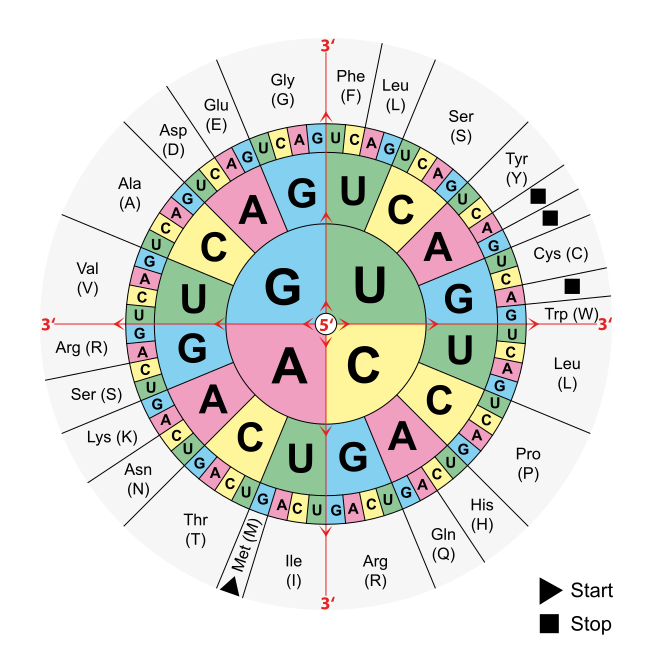
\includegraphics[width = 5 cm] {pictures/Aminoacids_table.png}	
				\end{figure}
			{\tiny Bildquelle: \cite{genetic_code}}
			% https://commons.wikimedia.org/wiki/File:Aminoacids_table.svg#/media/File:Aminoacids_table.svg
			\end{center}
		\end{column}
	\end{columns}
\end{frame}

\section{Biologischer Hintergrund}
\subsection{title}
\begin{frame}
	\frametitle{}
		\begin{block}{Proteinbiosyntese}
		\begin{itemize}
			\item �bersetzung der Basensequenz der DNA in die Aminos�uresequenz der Proteine
		\end{itemize}
		\begin{enumerate}[\begingroup\color{black} 1\endgroup]
		{\setlength{\itemindent}{1.5em}
%			\vspace{0.1cm}
			\visible<2->{\item \textbf{Transkription}:
			\item[] $\Rightarrow$ \textbf{Umschreiben} eines DNA-Abschnitts in RNA
			\item[] $\Rightarrow$ dadurch werden Arbeitskopien in Form von \textbf{mRNA} 
			\item[]\hspace{0.4cm} (messenger RNA) hergestellt}
%			\vspace{0.1cm}
			\visible<3->{
				\item \textbf{Translation}:
					\item[] $\Rightarrow$ \textbf{�bersetzen} der Basensequenz in die Aminos�uresequenz
					\item[] $\Rightarrow$ dadurch werden Arbeitskopien in Form von \textbf{mRNA} }
		}
		\vspace{0.4cm} 
	\end{enumerate}
	\end{block}
	%	\vspace {0.8cm}

\end{frame}






%%Folie 4
\section{}
\subsection{}
\begin{frame}
	\frametitle{}
	text
\end{frame}

%%Folie 5
\section{}
\subsection{}
\begin{frame}
	\frametitle{}
	text
\end{frame}

%%Folie 6
\section{}
\subsection{}
\begin{frame}
	\frametitle{}
	text
\end{frame}

%%Folie 7
\section{}
\subsection{}
\begin{frame}
	\frametitle{}
	text
\end{frame}


%%Folie 8
\section{}
\subsection{}
\begin{frame}
	\frametitle{}
	text
\end{frame}


%%Folie 9
\section{}
\subsection{}
\begin{frame}
	\frametitle{}
	text
\end{frame}


%%Folie 10
\section{}
\subsection{}
\begin{frame}
	\frametitle{}
	text
\end{frame}


%%Folie 11
\section{}
\subsection{}
\begin{frame}
	\frametitle{}
	text
\end{frame}


%%Folie 12
\section{}
\subsection{}
\begin{frame}
	\frametitle{}
	text
\end{frame}


%%Folie 13
\section{}
\subsection{}
\begin{frame}
	\frametitle{}
	text
\end{frame}


%%Folie 14
\section{}
\subsection{}
\begin{frame}
	\frametitle{}
	text
\end{frame}


%%Folie 15
\section{}
\subsection{}
\begin{frame}
	\frametitle{}
	text
\end{frame}


%%Folie 16
\section{}
\subsection{}
\begin{frame}
	\frametitle{}
	text
\end{frame}


%%Folie 17
\section{}
\subsection{}
\begin{frame}
	\frametitle{}
	text
\end{frame}


%%Folie 18
\section{}
\subsection{}
\begin{frame}
	\frametitle{}
	text
\end{frame}


%%Folie 19
\section{}
\subsection{}
\begin{frame}
	\frametitle{}
	text
\end{frame}


%%Folie 20
\section{}
\subsection{}
\begin{frame}
	\frametitle{}
	text
\end{frame}


%%Folie 21
\section{}
\subsection{}
\begin{frame}
	\frametitle{}
	text
\end{frame}


%%Folie 22
\section{}
\subsection{}
\begin{frame}
	\frametitle{}
	text
\end{frame}


%%Folie 23
\section{}
\subsection{}
\begin{frame}
	\frametitle{}
	text
\end{frame}


%%Folie 24
\section{}
\subsection{}
\begin{frame}
	\frametitle{}
	text
\end{frame}


%%Folie 25
\section{}
\subsection{}
\begin{frame}
	\frametitle{}
	text
\end{frame}


%%Folie 26
\section{}
\subsection{}
\begin{frame}
	\frametitle{}
	text
\end{frame}


%%Folie 27
\section{}
\subsection{}
\begin{frame}
	\frametitle{}
	text
\end{frame}


%%Folie 28
\section{}
\subsection{}
\begin{frame}
	\frametitle{}
	text
\end{frame}


%%Folie 29
\section{}
\subsection{}
\begin{frame}
	\frametitle{}
	text
\end{frame}


%%Folie 30
\section{}
\subsection{}
\begin{frame}
	\frametitle{}
	text
\end{frame}


%%Folie 31
\section{}
\subsection{}
\begin{frame}
	\frametitle{}
	text
\end{frame}


%%Folie 32
\section{}
\subsection{}
\begin{frame}
	\frametitle{}
	text
\end{frame}


%%Folie 33
\section{}
\subsection{}
\begin{frame}
	\frametitle{}
	text
\end{frame}


%%Folie 34
\section{}
\subsection{}
\begin{frame}
	\frametitle{}
	text
\end{frame}


%%Folie 35
\section{}
\subsection{}
\begin{frame}
	\frametitle{}
	text
\end{frame}


%%Folie 36
\section{}
\subsection{}
\begin{frame}
	\frametitle{}
	text
\end{frame}


%%Folie 37
\section{}
\subsection{}
\begin{frame}
	\frametitle{}
	text
\end{frame}


%%Folie 38
\section{}
\subsection{}
\begin{frame}
	\frametitle{}
	text
\end{frame}


%%Folie 39
\section{}
\subsection{}
\begin{frame}
	\frametitle{}
	text
\end{frame}


%%Folie 40
\section{}
\subsection{}
\begin{frame}
	\frametitle{}
	text
\end{frame}


%%Folie 41
\section{}
\subsection{}
\begin{frame}
	\frametitle{}
	text
\end{frame}


%%Folie 42
\section{}
\subsection{}
\begin{frame}
	\frametitle{}
	text
\end{frame}


%%Folie 43
\section{}
\subsection{}
\begin{frame}
	\frametitle{}
	text
\end{frame}


%%Folie 44
\section{}
\subsection{}
\begin{frame}
	\frametitle{}
	text
\end{frame}


%%Folie 45
\section{}
\subsection{}
\begin{frame}
	\frametitle{}
	text
\end{frame}


%%Folie 46
\section{}
\subsection{}
\begin{frame}
	\frametitle{}
	text
\end{frame}


%%Folie 47
\section{}
\subsection{}
\begin{frame}
	\frametitle{}
	text
\end{frame}


%%Folie 48
\section{}
\subsection{}
\begin{frame}
	\frametitle{}
	text
\end{frame}


%%Folie 49
\section{}
\subsection{}
\begin{frame}
	\frametitle{}
	text
\end{frame}


%%Folie 50
\section{}
\subsection{}
\begin{frame}
	\frametitle{}
	text
\end{frame}


%Literaturverzeichnis
\begin{frame}%[allowframebreaks]
	\frametitle{Bildquellen}
	\bibliographystyle{plain}
	\bibliography{bibliography/RAD-Seq_slices}
%	\addcontentsline{toc}{section}{\bibname}
\end{frame}

\end{document}